\chapter{Tensor energía-momento. Campo escalar}

	
\begin{tikzpicture}
	\fill [left color=red!50, right color=teal!50] (0,0) rectangle (6.5,.1);
	\fill [left color=teal!50, right color=blue!50] (6.5,0) rectangle (11.5,.1);
	\end{tikzpicture}


\vspace{10mm}
\begin{adjustwidth}{50pt}{50pt}
\begin{ejemplo}
Vamos a definir el tensor energía-momento para un campo clásico (también servirá para la versión cuántica) y lo haremos a través de la simetría continua de la traslación. Aplicaremos el teorema de Noether a esta simetría.

\end{ejemplo}
\end{adjustwidth}
\vspace{10mm}

\begin{ejemplo}
\underline{Aclaración}:  Para el lagrangiano de Klein-Gordon, 	$\mathcal L=\partial_\mu \phi \partial^\mu \phi - \dfrac{m^2}{2} \phi^2$, al calcular la ecuación de movimiento aplicando las ecuaciones de Euler-Lagrange, obtuvimos $\left(\partial_\mu \partial^\mu + m^2 \right) \phi = 0$.

En cambio, en el capítulo anterior el resultado que obtuvimos para la ecuación de Klein-Gordon era: $\left[\partial_\mu \partial^\mu + \left( \dfrac{mc}{\hbar} \right)^2 \right] \phi  = 0$

La explicación está en que al definir $\mathcal L$ lo hacíamos en el \emph{sistema natural de unidades} o \emph{sistema de Plank}, en que $\hbar=c=1$. Veremos esto en un próximo capítulo.
\end{ejemplo}

\vspace{5mm}
\section{Traslación espacio-temporal}

Consideremos un lagrangiano genérico, $\quad \boldsymbol{ \mathcal L=\dfrac 1 2 \partial_\mu \phi \ \partial^\mu \phi - U(\phi)}$

La acción será $\quad \boldsymbol{ s[\phi] \ = \ \displaystyle \int \dd^4 \ \mathcal L (\phi, \partial_\mu \phi) }$

\hspace{1cm} $\triangleright \quad$ Si $\ U(\phi)=\dfrac{m^2}2\phi^2 \ \to \ $ obtendríamos el campo de Klein-Gordon.

\hspace{1cm} $\triangleright \quad$ Ha de ocurrir que $\quad\begin{cases} \ \phi(\ |x|,\ |t| \ \to \ +\infty \  ) \ \sim \ 0 \\ \ \partial_\mu \phi(\ |x|,\ |t| \ \to \ +\infty \  ) \ \sim \ 0  \end{cases}$


\vspace{5mm}Vamos con una \textbf{traslación espacio-temporal}:

$x^\mu \ \to \ \widetilde{x^\mu} \ = \ x^\mu + a^\mu  \qquad \text{dim }(1+1)\, : \quad \begin{cases}\ c\tilde t = ct+a^0 \\ \ \tilde x=x+a^1 \end{cases}$

Podemos interpretar que se trata de otro observador que mide el mismo campo en el mismo punto: $\ \phi(x^\mu)= \tilde \phi(\tilde  x^\mu)$, en general, $\phi(x)=\tilde \phi(\tilde x)$. Esto solo es cierto para campos escalares.

\vspace{5mm}
\begin{ejemplo}
\underline{Importante}:

$\tilde \phi(\tilde x)=\phi(x) \ \to \ $ Podemos definir $\ \tilde \delta \phi=	\phi(\tilde x)-\phi(x) \quad \to \quad \tilde \delta \phi=0$

Puede haber situaciones en que $\tilde \delta \phi \neq 0$ y solo se darán para campos vectoriales (tensoriales).

En un campo escalar, $\ \tilde \delta \phi=\tilde \phi(\tilde x)-\phi(x)=0$. En un campo vectorial, $ \tilde \delta \phi_a=\tilde \phi_a(\tilde x)-\phi_a(x)$ puede ser distinto de cero. Un vector  tiene distintas componentes para cada observador.
\begin{multicols}{2}


$A=A^0e_0+A^1e_1=A^{0'}e_{0'}+A^{1'}e_{1'}\, , \ $ 

con $A^0\neq A^{0'} \ \wedge \ A^1\neq A^{1'}\, , \ $

por lo que $\ \tilde A=\tilde A^\mu_{(\tilde x)} - A^\mu_{(x)} \neq 0$

El campo escalar no depende de la base, el campo vetorial sí.

\emph{Los campos vectoriales darán lugar al spin.}

\begin{figure}[H]
	\centering
	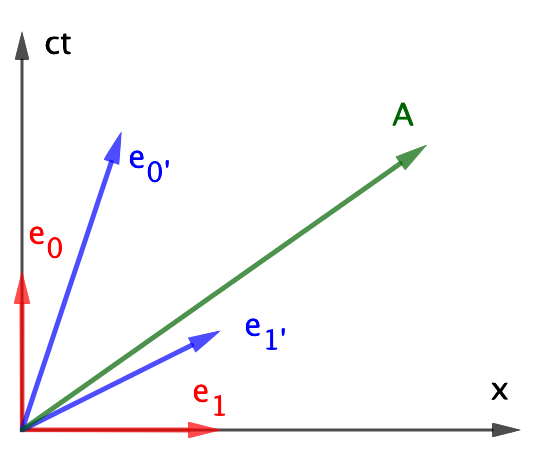
\includegraphics[width=.4\textwidth]{imagenes/img34-01.png}
\end{figure}
\end{multicols}
\end{ejemplo}

$\boldsymbol{ \phi(x) \ = \ \tilde \phi(\tilde x) } \quad $ \textbf{Campo escalar}, queda inalterado por una translación espacio-temporal.

Veamos como se transforma $\partial_\mu \phi$ en una
traslación espacio-temporal (1+1) dim: $\ \begin{cases} \ \tilde x^0=x^0+a^0 \\ \ \tilde x^1=x^1+a^1 \end{cases}$

$\displaystyle \partial_\mu \phi = \pdv{\phi}{x^\mu} \ \to \ $

\hspace{1cm}  $\displaystyle \partial_0 \phi = \pdv{\phi}{x^0}=\pdv{\tilde x^0}{x^0}\pdv{\phi}{\tilde x^0}+\pdv{\tilde x^1}{x^0}\pdv{\phi}{\tilde x^1}=1 \ \partial{\phi}{\tilde x^0}+0=\partial{\phi}{\tilde x^0}=\partial_{\tilde 0}\phi\, , \ $ 

\hspace{1cm} análogamente, $\displaystyle \ \partial_1 \phi=\pdv{\phi}{x^1}=\pdv{\phi}{\tilde x^1}=\partial_{\tilde 1} \phi $ por lo que $\partial_\mu \phi= \partial_{\tilde \mu} \phi$ y también $\partial^\mu \phi= \partial^{\tilde \mu} \phi$ 

Por ello, $ \ \partial_\mu \phi \  \partial^\mu \phi= \partial_{\tilde \mu} \phi \ \partial^{\tilde \mu} \phi \ $ es un invariante bajo traslaciones espacio-temporales así como el campo $\pi$ y, evidentemente, el potencial $U(\phi)$ por lo que la acción será también invariante: $\ \boldsymbol {S[\phi] \ = \ S[\tilde \phi]}$

\vspace{5mm} Para poder aplicar el teorema de Noether necesitamos una transformación infinitesimal: $\ a^\mu \ / \ (a^\mu)^2 \approx 0$

$\tilde \phi(\tilde x)=\phi(x) \ \ \to \ \ \tilde \phi (x^\mu+ a^\mu)=\phi(x) \ $ Aplicando un Taylor:

$\tilde \phi (x^\mu+ a^\mu) \approx \tilde \phi(x) + \displaystyle \pdv{\tilde \phi}{\tilde x^\mu} a^\mu  \approx \phi(x)$

Como $\tilde \phi(\tilde x)=\phi(x) \ \ \to \  \ \displaystyle \pdv{\tilde \phi}{\tilde x^\mu}=\pdv{x^\alpha}{\tilde x^\mu}\pdv{\tilde \phi}{x^\alpha}= \delta^\alpha_\mu \pdv{\tilde \phi}{x^\alpha}=\pdv{\tilde \phi}{x^\mu}$

Luego, $\ \displaystyle \tilde \phi(x^\mu)+ \displaystyle \pdv{\phi}{x^\mu} a^\mu = \tilde \phi (x^\mu) + \partial_\mu \phi a^\mu \approx \phi(x)$

$\tilde \phi  (x^\mu) + a^\mu \partial_\mu \phi \approx \phi(x) \ \to \ \tilde \phi(x^\mu)-\phi(x^\mu) \approx -a^\mu \partial_\mu \phi \ $ en general $\ \tilde \phi(x) - \phi(x) \approx -a^\mu \partial_\mu \phi(x)$

\textcolor{gris}{Ojo, $\ \phi(x)$ no es lo mismo que $\tilde \phi(x)$}

\vspace{5mm}
Hemos obtenido $\tilde \phi(\tilde x) = \phi(x) \ \to \ \tilde \phi(x)-\phi(x) \approx - a^\mu \partial_\mu \phi$
\begin{multicols}{2}
\begin{figure}[H]
	\centering
	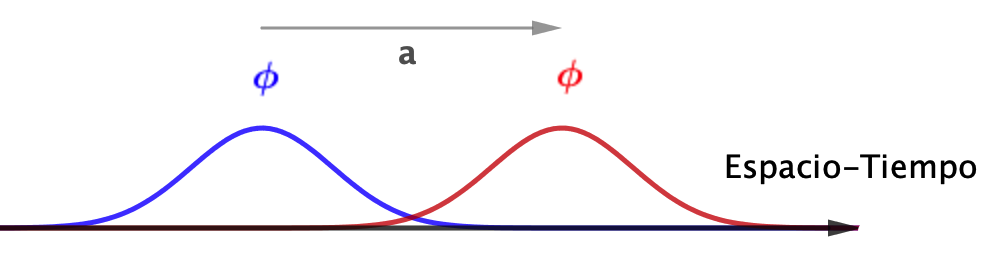
\includegraphics[width=.4\textwidth]{imagenes/img34-02.png}
\end{figure}
Se puede interpretar como una variación del campo:
$\ \ \boldsymbol{ \delta \phi=- a^\mu \partial_\mu \phi(x)}$
\end{multicols}
En lugar de una traslación espacio-temporal es como si hubiésemos hecho una traslación del campo (traslación activa).

Una traslación espacio-temporal, una transformación pasiva, puede verse como una traslación del campo, transformación activa. Ambos puntos de vista conducen a la misma conclusión. Y esto es válido para cualquier traslación espacio-temporal de cualquier campo escalar.

\vspace{5mm}
\begin{multicols}{2}
$\mathcal L(\phi, \partial_\mu \phi)$ no depende explícitamente de $x$ pero sí lo hacen el campo $\phi(x)$ y las derivadas $\partial_\mu(x)$, por lo que $\mathcal L(\phi(x), \partial_\mu \phi(x))$ y podremos asociar a cada punto espacio-temporal un valor para la densidad lagrangiana $\mathcal L$ e interpretarlo como que se trata de una 'superficie' en el espacio-tiempo.  Al hacer una traslación infinitesimal, $\mathcal L$ se comportará como lo hacen los campos: $\  \boldsymbol{ \delta \mathcal L=- a^\mu \partial_\mu \mathcal L}\ \ $ \textcolor{gris}{(Para una transformación finita sí ocurre que $\delta \mathcal L=0$, pero para una infinitesimal $\displaystyle \delta \mathcal L=- a^\mu \partial_\mu \mathcal L$ )}
 
\begin{figure}[H]
	\centering
	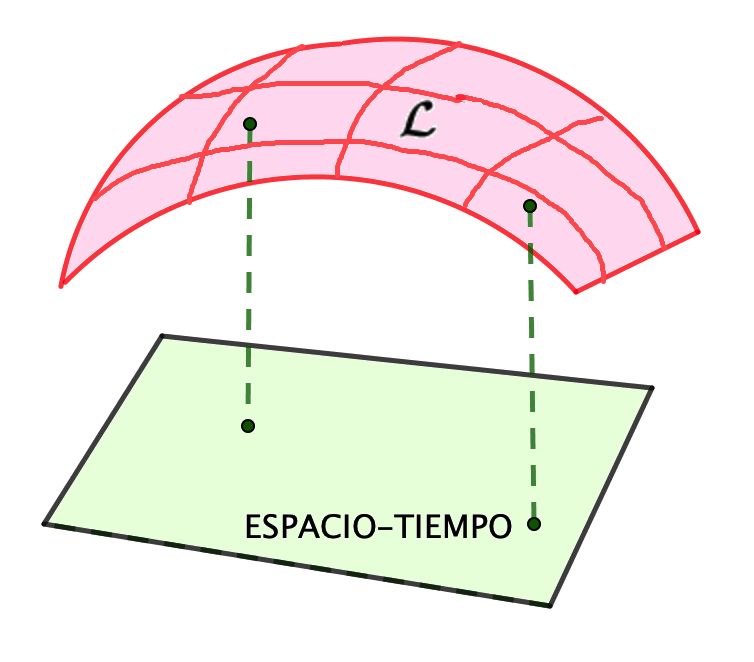
\includegraphics[width=.35\textwidth]{imagenes/img34-03.png}
\end{figure}
\end{multicols}

\textcolor{gris}{Lo que acabamos de ver es similar a lo que ya vimos con las transformaciones infinitesimales en el teorema de Noether, $\ \delta  L=\varepsilon \dv{K}{t}$, ahora, en teoría de campos, $\displaystyle \delta \mathcal L=- a^\mu \partial_\mu \mathcal L$} 


\section{Tensor energía momento}

El hecho de hacer una traslación espacio-temporal $\ \tilde x^\mu=x^\mu+a^\mu\ $ nos ha llevado a que el campo cambia en la forma 
$\ \delta \phi \approx -a^\mu \partial_\mu \phi \ $ y que la densidad lagrangiana cambia en el mismo modo,
$\ \delta \mathcal L\approx -a^\mu \partial_\mu \mathcal L\, . \ $ Volviendo a usar la misma nomenclatura que usábamos con las simetrías,

\hspace{2cm} $\boldsymbol{ (\delta \phi)_S \approx -a^\mu \partial_\mu \phi \qquad  \qquad (\delta \mathcal L)_S \approx -a^\mu \partial_\mu \mathcal L}$

También calculábamos el cambio del lagrangiano usando las ecuaciones de Euler-Lagrange, 

\hspace{2cm}$\displaystyle \boldsymbol{ (\delta \mathcal L)_{E-L} = \pdv{\mathcal L}{\phi} \delta \phi + \pdv{\mathcal L}{(\partial_\mu \phi)} \delta(\partial_\mu \phi)}$

Para calcular $\delta \phi=\tilde \phi(x)-\phi(x)$, lo hemos hecho en un mismo punto $x$ del espacio-tiempo, es por ello por lo que variación $\delta$ y derivación $\partial_\mu$  conmutan: $\ \delta(\partial_\mu \phi) = \partial_\mu(\delta \phi)$

\hspace{1cm} \textcolor{gris}{\underline {Ejemplo}: $\phi=e^{-x^2};\ \ \tilde \phi=\sin x \qquad \phi'=-2xe^{-x^2} ; \ \ \tilde \phi'=\cos x$}

\hspace{1cm} \textcolor{gris}{$\delta \phi'=\cos x + 2x e^{-x^2} ;\quad \delta \phi=\sin x - e^{-x^2} \ \to \ (\delta \phi)'= \cos x + 2xe^{-x^2}$}

Luego, $\quad \displaystyle (\delta \mathcal L)_{E-L} \ = \ \pdv{\mathcal L}{\phi} \ + \ \underbrace{ \pdv{\mathcal L}{(\partial_\mu \phi)} }_{A}  \underbrace{ \ \partial_\mu (\delta \phi) }_{B} \qquad $
Aplicando que $\ A\partial B=\partial(AB)-(\partial A)B$,

$\displaystyle  \pdv{\mathcal L}{(\partial_\mu \phi)}  \ \partial_\mu (\delta \phi) = \partial_\mu \left( \pdv{\mathcal L}{(\partial_\mu \phi)} \delta \phi \right) - \partial_\mu \left( \pdv{\mathcal L}{(\partial_\mu \phi)} \right) \delta \phi$ 

Sustituyendo en  $\ \  \displaystyle (\delta \mathcal L)_{E-L} \ = \pdv{\mathcal L}{\phi} \ \delta \phi \ + \  \partial_\mu \left( \pdv{\mathcal L}{(\partial_\mu \phi)} \ \delta \phi \right) \ - \ \partial_\mu \left( \pdv{\mathcal L}{(\partial_\mu \phi)} \right) \ \delta \phi$

Reordenando y sacando $\delta \phi$ factor común,

$(\delta \mathcal L)_{E_L} \ = \ \displaystyle
\cancelto{0,\ \begin{tiny}^\text{E-L}\end{tiny} }{
\left[ \pdv{\mathcal L}{\phi} - \partial_\mu \left( \pdv{\mathcal L}{(\partial_\mu \phi)} \right) \right]
} \delta \phi \ + \ 
\partial_\mu \left( \pdv{\mathcal L}{(\partial_\mu \phi)} \delta \phi \right)\ $ 

Término nulo, ya que estamos calculando la variación de la densidad lagrangiana suponiendo que se cumplen las ecuaciones de Euler-Lagrange.

\hspace{2cm} $\text{Por Euler-Lagranqe } \quad \quad \boldsymbol{ (\delta \mathcal L)_{E-L} \ = \ \displaystyle
\partial_\mu \left( \pdv{\mathcal L}{(\partial_\mu \phi)} \ \delta \phi \right)\ }$

\hspace{2cm} $\text{Por la simetría } \qquad \qquad \boldsymbol{(\delta \mathcal L)_S \ = \ -a^\mu \ \partial_\mu \mathcal L}$

Ambas variaciones no son lo mismo, pero si imponemos que $\delta \phi$ sea siguiendo la simetría, $(\delta \phi)_S$, entonces ambas expresiones sí son iguales y el \emph{teorema de Noether} dice que:


$$  \displaystyle \boldsymbol{
\partial_\mu \left( \pdv{\mathcal L}{(\partial_\mu \phi)} \ (\delta \phi)_S \right)\ 
= \ \ -a^\mu \ \partial_\mu \mathcal L}$$

Como vimos anteriormente, $\ (\delta \phi)_S\ = \ -a^\mu \ \partial \mu \phi \ $, sustituyendo,

$$  \displaystyle \boldsymbol{\partial_\mu \left( \pdv{\mathcal L}{(\partial_\mu \phi)} \ a^\mu \ \partial_\mu \phi  \right)\ = \ \ a^\mu \ \partial_\mu \mathcal L}$$

Todo a la izquierda, $\quad \displaystyle \partial_\mu \left( \pdv{\mathcal L}{(\partial_\mu \phi)} \ a^\mu \ \partial_\mu \phi  \right)\ -  \ a^\mu \ \partial_\mu \mathcal L \ = 0\, , \ $ poniendo un poco de orden el los índices,

$\displaystyle \partial_\mu \left( \pdv{\mathcal L}{(\partial_\mu \phi)} \ a^\alpha \ \partial_\alpha \phi  \right)\ -  \ a^\beta \ \partial_\beta \mathcal L \ = 0\, . \quad $
Hacemos ahora $\ \beta=\mu\ $ para poder simplificar la expresión $\quad$ ($\beta$ es un índice mudo) y, por otra parte,  como $a^\mu=cte \ \to \ a^\mu \partial_\mu \mathcal L=\partial_\mu (a^\mu \mathcal L)$, podemos sacar factor común y escribir:

$\displaystyle \partial_\mu \left( \pdv{\mathcal L}{(\partial_\mu \phi)} \ a^\alpha \partial_\alpha \phi \right) \ - \ \partial_\mu(a^\mu \mathcal L) \ = \ 0 \quad \to \qquad
 \partial_\mu \left[ \left( \pdv{\mathcal L}{(\partial_\mu \phi)} \ a^\alpha \partial_\alpha \phi \right) \ - \ a^\mu \mathcal L \right] \ = \ 0$ 
 
 En esta expresión no podemos hacer $\alpha=\mu$ pues $\alpha$ no es índice mudo, pero si podemos usar la identidad $\ a^\mu=\delta^\mu_\alpha a^\alpha$ y escribir
 
$\displaystyle  \partial_\mu \left[ \left( \pdv{\mathcal L}{(\partial_\mu \phi)} \ a^\alpha \partial_\alpha \phi \right) \ - \ \delta^\mu_\alpha a^\alpha \mathcal L \right] \ = \ 0 \quad \to \quad 
a^\alpha \partial\mu \left[ \left( \pdv{\mathcal L}{(\partial_\mu \phi)} \  \partial_\alpha \phi \right) \ - \ \delta^\mu_\alpha \mathcal L \right] \ = \ 0\, ; \quad a^\alpha \neq 0 \Rightarrow$  

\vspace{5mm}
\begin{large}
\begin{myblock}{$\qquad T^\mu_\alpha \ \textit{ tensor energía momento del campo}$}
\begin{equation}
\label{T34TEMC}
\boldsymbol{ \boxed{ \ 
\partial\mu \left[ \left( \pdv{\mathcal L}{(\partial_\mu \phi)} \  \partial_\alpha \phi \right) \ - \ \delta^\mu_\alpha \mathcal L \right] \ = \partial_\mu \ T^\mu_\alpha \ = \ 0	 \ } } \
\end{equation}
\end{myblock}
\end{large}

\vspace{5mm}
\begin{destacado}
En toda teoría de campos, $\ \begin{cases} \ \mathcal L=\dfrac 1 2 \partial_\mu \phi \partial^\mu \phi \\ \ S[\phi]=\displaystyle \int \dd^4 x \ \mathcal L(\phi, \partial_\mu \phi) \end{cases} \ $	 siempre se puede definir un tensor energía momento $\ \displaystyle T^\mu_\alpha \ = \ \left( \pdv{\mathcal L}{(\partial_\mu \phi)} \  \partial_\alpha \phi \right) \ - \ \delta^\mu_\alpha \mathcal L \ $ tal que su divergencia sea nula, $\ \partial_\mu T_\alpha^\mu \ = \ 0$
\end{destacado}
\vspace{5mm}

Normalmente, el tensor energía momento viene definido con los índices arriba:

\begin{definition}
.	\begin{equation}
	\label{T34TEMcontra}	
	\boldsymbol{ T_{\mu \nu} } \ = \ \ g^{\nu \alpha} \ T^\mu_\alpha \ \ = \ \displaystyle \boldsymbol{ \pdv{\mathcal L}{(\partial_\mu \phi)} \  \partial^\mu \phi  \ - \ g^{\mu \nu} \mathcal L }. \qquad \qquad \boldsymbol{\partial_\mu T^{\mu \nu} = \ 0}
	\end{equation}
\end{definition}

\begin{center}\textcolor{gris}{($\ g^{\nu \alpha} \partial_\alpha \ = \ \partial^\nu \qquad \qquad\qquad g^{\nu \alpha} \delta^\mu_\alpha=g^{\nu \mu}=g^{\mu \nu}\, , \ g^{\mu \nu}\ $ tensor simétrico. )}\end{center}

\vspace{5mm} Vamos a calcular las componentes del tensor energía momento, para ello, escribiremos $\mathcal L$ de modo más cómodo como:

$\mathcal L=\dfrac 1 2 \partial_\mu \phi \partial^\mu \phi - U(\phi)=\dfrac 1 2 \left( (\partial_0 \phi)^2-(\partial_1 \phi)^2-(\partial_2 \phi)^2-(\partial_3 \phi)^2 \right) - U(\phi)$

Es costumbre llamar $\ \dot \phi=\partial_0 \phi\ $ por lo que $\ \boldsymbol{ \mathcal L= \dfrac 1 2 \dot \phi^2- \dfrac 1 2 (\partial_1 \phi)^2-\dfrac 1 2 (\partial_2 \phi)^2-\dfrac 1 2 (\partial_3 \phi)^2 - U(\phi)} \ $

\textcolor{gris}{Recordar que $\ \ \partial^0=\partial_0 \quad \partial^i=-\partial_i\, , \ i=1,2,3$}

\vspace{5mm}
\textbf{Componentes del tensor energía momento}:

$\triangleright \qquad \displaystyle T^{00}=\dot \phi \ \cancelto{ \partial_0 \phi=\dot \phi}{\partial^0} \phi \ - \  \cancelto{1}{g^{00}} \mathcal L = \dot \phi^2-\dfrac 1 2 \dot \phi^2+ \dfrac 1 2 (\partial_1 \phi)^2+\dfrac 1 2 (\partial_1 \phi)^2+\dfrac 1 2 (\partial_1 \phi)^2 + U(\phi)$ 

Llamando $\quad\overrightarrow \nabla \phi=(\partial_1\phi,\partial_2\phi,\partial_2\phi)\, \ $ gradiente espacial del campo,
 
$\boldsymbol{T^{00} \ = \ \dfrac 1 2 \dot \phi^2 \ + \dfrac 1 2 (\overrightarrow \nabla \phi)^2 \ + \  \ U(\phi)} \quad \sim \ \textbf{energía} \qquad $ \begin{tiny}$U(\phi) \text{ término potencial, } + \ \dfrac12\partial_\mu \phi \partial^\mu \phi + \dfrac 1 2 (\overrightarrow \nabla \phi)^2 \text{ término cinético}$\end{tiny}

La componente $T^{00}$ del tensor energía-momento se  llama 	\textbf{\emph{densidad de energía}} y se representa por:

\begin{adjustwidth}{30pt}{30pt}
\begin{myalertblock}{Densidad de energía}
\begin{large}
\begin{equation}
\label{T34dens-energia}	
\boldsymbol{ 
\mathcal H \ = \ T^{\ 00} \ = \  \dfrac 1 2 \dot \phi^2 \ + \dfrac 1 2 (\overrightarrow \nabla \phi)^2 \ + \  \ U(\phi)
}
\end{equation}
\end{large}
\end{myalertblock}
\end{adjustwidth}


\vspace{3mm} $\triangleright \qquad \displaystyle T^{01}=\dot \phi \ \partial^1 \phi - 0 = - \dot \phi \ \partial_1 \phi \qquad \to \qquad \boldsymbol{ T^{0i}\ = \ -\dot \phi \ \partial_i \phi}\quad i=1,2,3$

\vspace{3mm} $\triangleright \qquad \displaystyle T^{10}=\partial{\mathcal L}{(\partial_1 \phi)} \ \partial^0\phi \ - \ 0 = -\dfrac 1 2 2 (\partial_1 \phi)\  \partial^0 \phi =-\partial_1 \phi \ \dot \phi=-\dot \phi \ \partial_1 \phi = T^{01} \quad \to \quad \boldsymbol {T^{i0}=T^{0i}}=-\dot \phi \ \partial_i\phi$


------ Como parece que $T^{\mu \nu}$ va a ser un tensor simétrico, comprobémoslo:

\hspace{.5cm} $T^{\alpha \beta}=T^{\beta \alpha} \quad \leftrightarrow \quad \displaystyle
\pdv{\mathcal L}{(\partial_\alpha \phi)} \ \partial^\beta \phi  - g^{\alpha \beta }  \mathcal L =
\pdv{\mathcal L}{(\partial_\beta \phi)} \ \partial^\alpha \phi  - g^{\beta \alpha }  \mathcal L\ $ 

\hspace{.5cm} como $ g^{\alpha \beta}=g^{\beta \alpha} \ $ (la métrica es simétrica), ha de ocurrir que:
$\quad \displaystyle 
\pdv{\mathcal L}{(\partial_\alpha \phi)} \ \partial^\beta \phi   =
\pdv{\mathcal L}{(\partial_\beta \phi)} \ \partial^\alpha \phi $

\hspace{1.5cm} $\left. \begin{matrix}
 	\displaystyle \pdv{\mathcal L}{(\partial_\alpha \phi)} \ \partial^\beta \phi  &  =\ \dfrac 1 2 \partial_\alpha \ \partial^\beta \phi \ 
 	\\ 
 	\displaystyle \pdv{\mathcal L}{(\partial_\beta \phi)} \ \partial^\alpha \phi  & = \  \dfrac 1 2 \partial_\beta \ \partial^\alpha \phi \ 
 \end{matrix} \right\} \ \text{ son iguales}$ $\qquad \qquad  \boldsymbol{ T^{\mu \nu} }\ $ es \textbf{simétrico} \hspace{2cm} $\Box$


\vspace{3mm} $\triangleright \qquad \displaystyle T^{ij}\, , \ \text{con } i \neq j\, : \qquad \boldsymbol{ T^{ij}} =
\pdv{\mathcal L}{(\partial_i \phi)} \partial^j \phi - \cancelto{0}{g^{ij}} \mathcal L =\dfrac 1 2 \partial_i \phi \ \partial^j \phi =
\boldsymbol{ - \dfrac 1 2 \partial_i \phi \ \partial_j \phi \ = \ T^{ji}}$

\vspace{3mm} $\triangleright \qquad i=i \ \to \ \displaystyle T^{ii} =
\pdv{\mathcal L}{(\partial_i \phi)} \partial^i \phi - \cancelto{1}{g^{ii}} \mathcal L = - \dfrac 1 2 \partial_i \phi \ \partial^i \phi + \mathcal L = \dfrac 1 2 (\partial_i \phi)^2 + \mathcal L =$

$T^{11} =  \displaystyle  \cancel{\dfrac 1 2 (\partial_1 \phi)^2} + \dfrac 1 2 \dot \phi^2- \cancel{ \dfrac 1 2 (\partial_1 \phi)^2}-\dfrac 1 2 (\partial_2 \phi)^2-\dfrac 1 2 (\partial_3 \phi)^2 - U(\phi) $

Expresión que, en general, podemos escribir como: $\displaystyle \dfrac 1 2 (\partial_i \phi)^2 - \sum_{k=1}^3 \dfrac 1 2 (\partial_k \phi)^2 = -\dfrac (1-\delta^j_i) (\partial_j \phi)^2\, , \ $ así,

$\boldsymbol{T^{ii} \ = \ \dfrac 1 2 (\partial_i \phi)^2 \ - \ \dfrac 1 2 (1-\delta^j_i) (\partial_j \phi)^2 \ - \ U(\phi)}$

\vspace{5mm}

\underline{Componentes del tensor energia momento}:

\begin{adjustwidth}{20pt}{20pt}

\color{NavyBlue}

$ \boldsymbol{ T^{00} \ = \ \dfrac 1 2 \dot \phi^2 \ + \dfrac 1 2 (\overrightarrow \nabla \phi)^2 \ + \   U(\phi) }$ 

$ \boldsymbol{T^{11} \ = \ \dfrac 1 2 \dot \phi^2 \ + \ \dfrac 1 2 (\partial_1 \phi)^2 \ - \ \dfrac 1 2 (\partial_2 \phi)^2 \ - \ \dfrac 1 2 (\partial_3 \phi)^2  \ - \ U(\phi)}$

$ \boldsymbol{T^{22} \ = \ \dfrac 1 2 \dot \phi^2 \ - \ \dfrac 1 2 (\partial_1 \phi)^2 \ + \ \dfrac 1 2 (\partial_2 \phi)^2 \ - \ \dfrac 1 2 (\partial_3 \phi)^2  \ - \ U(\phi)}$

$ \boldsymbol{T^{33} \ = \ \dfrac 1 2 \dot \phi^2 \ - \ \dfrac 1 2 (\partial_1 \phi)^2 \ - \ \dfrac 1 2 (\partial_2 \phi)^2 \ + \ \dfrac 1 2 (\partial_3 \phi)^2  \ - \ U(\phi)}$

$ \boldsymbol{T^{0i} \ = \ T^{i0} = - \dot \phi \ \partial_i \phi } \qquad i=1,2,3$

$ \boldsymbol{T^{12}\ = \ T^{21} \ = \ \partial_1 \phi \partial_2 \phi}\, ,  \qquad
\boldsymbol{T^{13}\ = \ T^{31} \ = \ \partial_1 \phi \partial_3 \phi}\, ,  \qquad \boldsymbol{T^{23}\ = \ T^{32} \ = \ \partial_2 \phi \partial_3 \phi}$
\end{adjustwidth}

\begin{comment} NO CABE todo el tensor
\begin{tiny}
$T^{\mu \nu} \ = \ 
\left( \ \begin{matrix}
\dfrac 1 2 \dot \phi^2 \ + \dfrac 1 2 (\overrightarrow \nabla \phi)^2 \ + \   U(\phi)&  - \dot \phi \ \partial_1 \phi&  - \dot \phi \ \partial_1 \phi&  - \dot \phi \ \partial_1 \phi \\	
 - \dot \phi \ \partial_1 \phi&  \dfrac 1 2 \dot \phi^2 \ + \ \dfrac 1 2 (\partial_1 \phi)^2 \ - \ \dfrac 1 2 (\partial_2 \phi)^2 \ - \ \dfrac 1 2 (\partial_3 \phi)^2  \ - \ U(\phi) && \\
 - \dot \phi \ \partial_2 \phi&& \dfrac 1 2 \dot \phi^2 \ - \ \dfrac 1 2 (\partial_1 \phi)^2 \ + \ \dfrac 1 2 (\partial_2 \phi)^2 \ - \ \dfrac 1 2 (\partial_3 \phi)^2  \ - \ U(\phi)& \\
 - \dot \phi \ \partial_3 \phi&&&  \dfrac 1 2 \dot \phi^2 \ - \ \dfrac 1 2 (\partial_1 \phi)^2 \ - \ \dfrac 1 2 (\partial_2 \phi)^2 \ + \ \dfrac 1 2 (\partial_3 \phi)^2  \ - \ U(\phi)
\end{matrix} \ \right)$
\end{tiny}
\end{comment}

\color{black}
\vspace{1cm}

Volvamos al lagrangiano de Klein-Gordon en (1+1)-dim, $(ct,x) \qquad \mathcal L = \dfrac 1 2 \dot \phi^2 - \dfrac 1 2 {\phi'}^2-\dfrac m 2 \phi^2$

En este caso, la densidad d energía es: $\qquad \mathcal H=T^{00}=\dfrac 1 2 \dot \phi^2 + \dfrac 1 2 {\phi'}¨2+\dfrac m 2 \phi^2$

?`Tendrá sentido definir la energía como $\ \text{Energía}=\displaystyle \int \dd x \ T^{00}=\int \dd x \ \mathcal H \ $?, integrando solo sobre la parte espacial, $\dd x$. Siendo $\phi$ solución de la ecuación de Klein-Gordon $\ (\partial_\mu \partial^\mu + m^2)\ \phi=0 \, , \ $ en nuestro caso (1+1)-dim, $\ (\partial_0^2-\partial_1^2+m^2)\phi=0 \ \to \ \boldsymbol{ \ddot \phi - \phi'' +m^2\phi=0}$

Solo podemos usar los campos que cumplan la ecuación anterior para sustituir en la expresión de la Energía que estamos testeando, campos que cumplirán la ecuación de Klein-Gordon y, además, habiendo simetría de traslación espacio-temporal ya que $\mathcal L=\mathcal L(\phi, \partial_\mu \phi)$

Imponemos también la condición del principio del tema, \begin{footnotesize}$\ \ \begin{cases} \ \phi(\ |x|,\ |t| \ \to \ +\infty \  ) \ \sim \ 0 \\ \ \partial_\mu \phi(\ |x|,\ |t| \ \to \ +\infty \  ) \ \sim \ 0  \end{cases} $\end{footnotesize} $ \phi, \ \dot \phi, \ \phi' \sim 0 \ \ (*)$ El campo y sus derivadas tienden a cero bien en los bordes del espacio-tiempo.

$\displaystyle H \ = \ \int_{-\infty}^{+\infty} \dd x \ \mathcal H \ = \ \int_{-\infty}^{+\infty} \dd x  \ \left( \dfrac 1 2 \dot \phi^2 + \dfrac 1 2 {\phi'}¨2+\dfrac m 2 \phi^2 \right)\ \ $ Si esto es la energía, como tenemos invarianza espacio-temporal, en concreto invarianza en el tiempo, deberá ocurrir que $\ \displaystyle \dv{H}{t} \ = \ 0 \ $ ?`Es esto cierto?

\textcolor{gris}{ Recordemos que $\ \ \displaystyle \dv{t} \int_a^b \dd x \ = \ \int_a^b \dd x \ \pdv{t} $}

\vspace{3mm}

$\displaystyle \dv{H}{t}=\int \pdv{t} \left( \dfrac 1 2 \dot \phi^2 + \dfrac 1 2 {\phi'}^2 + \dfrac m 2 \phi^2 \right) \ \dd x = \int \dd x \ (\dot \phi \ddot \phi + \phi' \dot{\phi'} + m^2 \phi \dot \phi) $

Al ser $\phi$ K-G $ \ \to \ \ddot \phi - \phi'' + m^2 \phi=0 \ \to \ m\phi^2=\phi''-\ddot \phi$

$\displaystyle \dv{H}{t}=  \int \dd x \ ( \dot \phi \ddot \phi + \phi' \dot{\phi'} + (\phi''-\ddot \phi) \ \dot \phi )=
\int \dd x \ ( \dot \phi \ddot \phi + (\phi''-\ddot \phi) \ \dot \phi + \phi' \dot{\phi'}  )=$
$\displaystyle \int \dd x \  [ \dot \phi \ (\cancel{\ddot \phi} + \phi'' - \cancel{\ddot \phi} ) + \phi' \dot{\phi'} ]   $

$\displaystyle \dv{H}{t}=\int \dd x \ \left( \  \underbrace{ \phi'\ '}_{A'}  \ \underbrace{\dot \phi}_{B} \ + \  \underbrace{\phi'}_{A} \  \underbrace{\dot{\phi \ '}}_{B'} \  \right) = \int_{-\infty}^{+\infty} \dd x \ \partial_x \ (\phi' \cdot \dot \phi ) = \eval{\phi' \cdot \dot \phi \ }_{-\infty}^{+\infty} = 0 \quad (*) \, , \ $ efectivamente.

La energía, en una determinada región del espacio, no del espacio-tiempo, en general no es cero (en todo el espacio, sí): $\ \displaystyle \dv{H}{t}=\int_a^b \dd x \ \partial_x (\phi' \dot \phi)=\eval{\phi' \cdot \dot \phi \ }_{a}^{b} \neq 0$


?`Entra esto en contradicción con el teorema de Noether? NO, Noether dice $\ \partial_\mu T^{\mu \nu} = 0 $, en nuestro caso, 
$\partial_0 T^{0\nu}+\partial_1 T^{1\nu}=0$. Para que aparezca $T^{00}$ hacemos $\nu=0$

$\partial_0 T^{00}+\partial_1 T^{10}=0 \ \to \ \partial_0 T^{00}=\partial_0 \mathcal H = \boldsymbol{ \partial_t \mathcal H} = - \partial_1 T^{10}= \boldsymbol{ -\partial_x T^{10} }$


En nuestros cálculo, $\ \displaystyle \dv{H}{t}=\int \dd x \ \partial_o T^{00}=-\int_a^b \dd x \ \partial_x (T^{01})\, , º  $ pero $\ T^{0i}=- \dot \phi \ \partial_i \phi \ \to \ T^{01} = - \dot \phi \ \phi'$

Luego $\displaystyle \ \dv{H}{t}=\int _a^b \dd x \ \partial_x (-T^{01})=-\int_a^b \dd x \ \partial_x T^{01}\, , \ $ de donde $\ \boldsymbol{\partial_o T^{00} = -\partial_1 T^{01}}$ que es lo que dice el teorema de Noether.

En una teoría de campos, la energía en una región localizada del espacio puede cambiar siguiendo la fórmula $\displaystyle \dv{H}{t}=-\int_a^b \dd x \ \partial_x T^{01} =\eval{-T^{01}}_b^a\, , \ $ depende de los extremos de la región espacial.

\vspace{1cm} Vamos a generalizarlo a 4-dimensiones y sin exigir que el campo sea de Klein-Gordon para mayor generalidad.

(3+1)-dim: $\quad \displaystyle \mathcal L=\dfrac 1 2 \dot \phi^2 - \dfrac 1 2  \dot{\phi'}^2-U(\phi);\quad \mathcal H=\dfrac 1 2 \dot \phi^2 + \dfrac 1 2  \dot{\phi'}^2+U(\phi); \quad \text{Energía}=\int \dd^3x \ T^{00}=-\int \dd^3 x \ \mathcal H$

\begin{multicols}{2}

$S$ superficie que envuelve a $V$; $\hat n$ perpendicular a $S$

$\qquad \displaystyle \dv{\text{ Energía}}{t}=\int \dd^3 x \ \partial_o T^{00}= (\to)$
\begin{figure}[H]
	\centering
	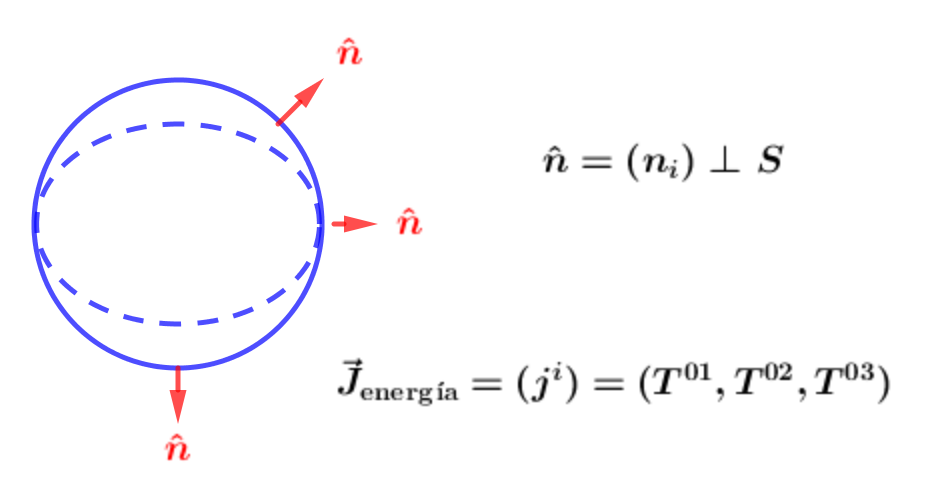
\includegraphics[width=.4\textwidth]{imagenes/img34-04.png}
\end{figure}
\end{multicols}

The. Noether: $\ \partial_0 T^{00}+\partial_1 T^{01}+\partial_2 T^{02}+\partial_2 T^{03} = 0 \ \to \ \partial_0 T^{00} = -\partial_1 T^{01}-\partial_2 T^{02}-\partial_2 T^{03}$

$\displaystyle (\to)= \int \dd^3 x \ ( -\partial_1 T^{01}-\partial_2 T^{02}-\partial_2 T^{03} ) = - \int_V \dd^3 x \ \partial_i T^{0i} = \textcolor{gris}{(\ \text{th. divergencia} \ )} = \int_{S(V)} \dd S \ n_i \ T^{0i}$

Llamamos \emph{\textbf{corriente de energía}}, $\vec J=(j^i)=(T^{01},T^{02},T^{02})$, indica como fluye la energía a través de las paredes de una región del espacio.

$$\displaystyle \displaystyle \dv{\text{ Energía}}{t}= -\int_V \dd^3 x \ \partial_i T^{0i} = - \int_{S(V)} \dd S \ n_i \ T^{0i} = -\int_{S(V)} \dd S \ \hat n \cdot \vec J_{\text{energía}}$$

Si en la expresión anterior cambiamos el índice $0$ por $1$, ya no estaremos hablando de la variación de la energía sino de otra cosa: se trata del momento lineal en la dirección $x$, en este caso., así:

$$\displaystyle \displaystyle \dv{\text{ Momento lineal - x}}{t}= \textcolor{gris}{ \left( \int \dd^3 x \ \partial_0 T^{10}  \right) } = 
-\int_V \dd^3 x \ \partial_i T^{1i} = - \int_{S(V)} \dd S \ n_i \ T^{1i} $$

Ahora, $\ \vec J_{ \text{ Momento lineal-x}} \ = \ (T^{11},T^{12},T^{13}) \ \ $ es la llamada \emph{corriente de la cantidad de movimiento} en la dirección $x$.

Para cualquiera de las tres direcciones espaciales, $k$,

$$\displaystyle \displaystyle \dv{\text{ Momento lineal - k}}{t}= \textcolor{gris}{ \left( \int \dd^3 x \ \partial_0 T^{k0}  \right) } = 
-\int_V \dd^3 x \ \partial_i T^{ki} = - \int_{S(V)} \dd S \ n_i \ T^{ki}\, ; \ \quad k=1,2,3$$

Con $ \ \vec J_{ \text{ Momento lineal -k}} \ = \ (T^{ki}) \ = \ (T^{k1},T^{k2},T^{k3}) \ $ es la \emph{corriente de la cantidad de movimiento} en la dirección $x$.


\vspace{5mm} \underline{Resumen}:


\begin{figure}[H]
	\centering
	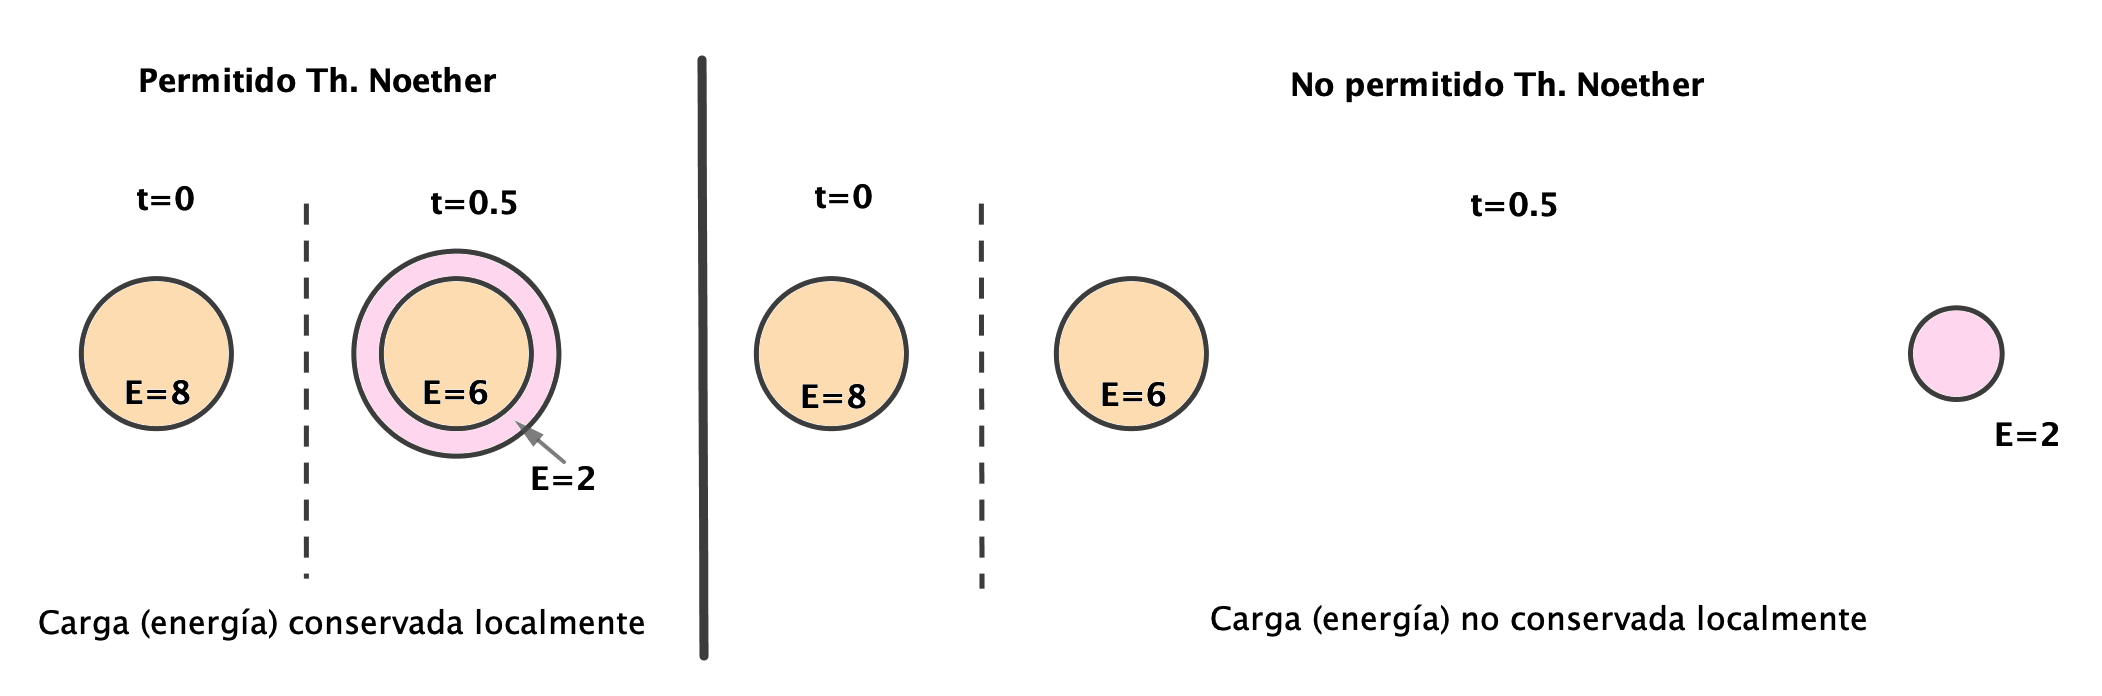
\includegraphics[width=.95\textwidth]{imagenes/img34-05.png}
\end{figure}


El teorema de Noether asegura que para cada simetría continua hay una carga conservada \emph{localmente}, en una cierta región del espacio. Lo que no permite el teorema es la segunda de las circunstancias representada en la figura superior, donde no hay conservación local de la carga (energía, p e ).


Para una \emph{simetría continua de traslación} y para un \emph{campo escalar} $\phi$ $\quad \Rightarrow \quad \exists $ tensor $\ T^{\mu \nu} \ $ tal que su divergencia es nula, $\ \partial_\mu T^{\mu \nu} = 0\ $ y existen \emph{$4$ leyes de conservación local} o \emph{$4$ corrientes conservadas}: $\ \partial_0 T^{\alpha 0}+ \partial_1 T^{\alpha 1}+ \partial_2 T^{\alpha 2}+ \partial_3 T^{\alpha 3} =0 \, ,  \quad \alpha=0,1,2,3$ 

\textcolor{gris}{$( \ \text{Ecuación de continuidad: } \ \partial_o \rho + \overrightarrow \nabla \cdot \vec J = 0 \ ) $}


\vspace{1cm}
\begin{adjustwidth}{60pt}{60pt}
\begin{destacado}
\vspace{2mm}

\color{NavyBlue}
\hspace{.5cm}\textbf{Corriente de energía}

\hspace{1cm} $\boldsymbol{ \partial_0 T^{0 0}+ \partial_1 T^{0 1}+ \partial_2 T^{02}+ \partial_3 T^{03} =0}$


\hspace{.5cm}\textbf{Corrientes de momento lineal}

\hspace{1cm} $\boldsymbol{ \partial_0 T^{10}+ \partial_1 T^{11}+ \partial_2 T^{12}+ \partial_3 T^{13} =0}$


\hspace{1cm} $\boldsymbol{ \partial_0 T^{20}+ \partial_1 T^{21}+ \partial_2 T^{22}+ \partial_3 T^{23} =0}$

\hspace{1cm} $\boldsymbol{ \partial_0 T^{30}+ \partial_1 T^{31}+ \partial_2 T^{32}+ \partial_3 T^{33} =0}$

$$\boldsymbol{ T^{00}=\mathcal H \, ; \quad T^{10}=\mathcal P^1 \ ; \quad  T^{20}=\mathcal P^2 \ ; \quad T^{30}=\mathcal P^3 }$$



\vspace{2mm}
\end{destacado}
\end{adjustwidth}
\color{black} 

